% Options for packages loaded elsewhere
\PassOptionsToPackage{unicode}{hyperref}
\PassOptionsToPackage{hyphens}{url}
\documentclass[
  ignorenonframetext,
]{beamer}
\newif\ifbibliography
\usepackage{pgfpages}
\setbeamertemplate{caption}[numbered]
\setbeamertemplate{caption label separator}{: }
\setbeamercolor{caption name}{fg=normal text.fg}
\beamertemplatenavigationsymbolsempty
% remove section numbering
\setbeamertemplate{part page}{
  \centering
  \begin{beamercolorbox}[sep=16pt,center]{part title}
    \usebeamerfont{part title}\insertpart\par
  \end{beamercolorbox}
}
\setbeamertemplate{section page}{
  \centering
  \begin{beamercolorbox}[sep=12pt,center]{section title}
    \usebeamerfont{section title}\insertsection\par
  \end{beamercolorbox}
}
\setbeamertemplate{subsection page}{
  \centering
  \begin{beamercolorbox}[sep=8pt,center]{subsection title}
    \usebeamerfont{subsection title}\insertsubsection\par
  \end{beamercolorbox}
}
% Prevent slide breaks in the middle of a paragraph
\widowpenalties 1 10000
\raggedbottom
\AtBeginPart{
  \frame{\partpage}
}
\AtBeginSection{
  \ifbibliography
  \else
    \frame{\sectionpage}
  \fi
}
\AtBeginSubsection{
  \frame{\subsectionpage}
}
\usepackage{iftex}
\ifPDFTeX
  \usepackage[T1]{fontenc}
  \usepackage[utf8]{inputenc}
  \usepackage{textcomp} % provide euro and other symbols
\else % if luatex or xetex
  \usepackage{unicode-math} % this also loads fontspec
  \defaultfontfeatures{Scale=MatchLowercase}
  \defaultfontfeatures[\rmfamily]{Ligatures=TeX,Scale=1}
\fi
\usepackage{lmodern}
\ifPDFTeX\else
  % xetex/luatex font selection
\fi
% Use upquote if available, for straight quotes in verbatim environments
\IfFileExists{upquote.sty}{\usepackage{upquote}}{}
\IfFileExists{microtype.sty}{% use microtype if available
  \usepackage[]{microtype}
  \UseMicrotypeSet[protrusion]{basicmath} % disable protrusion for tt fonts
}{}
\makeatletter
\@ifundefined{KOMAClassName}{% if non-KOMA class
  \IfFileExists{parskip.sty}{%
    \usepackage{parskip}
  }{% else
    \setlength{\parindent}{0pt}
    \setlength{\parskip}{6pt plus 2pt minus 1pt}}
}{% if KOMA class
  \KOMAoptions{parskip=half}}
\makeatother
\usepackage{longtable,booktabs,array}
\newcounter{none} % for unnumbered tables
\usepackage{calc} % for calculating minipage widths
\usepackage{caption}
% Make caption package work with longtable
\makeatletter
\def\fnum@table{\tablename~\thetable}
\makeatother
\usepackage{graphicx}
\makeatletter
\newsavebox\pandoc@box
\newcommand*\pandocbounded[1]{% scales image to fit in text height/width
  \sbox\pandoc@box{#1}%
  \Gscale@div\@tempa{\textheight}{\dimexpr\ht\pandoc@box+\dp\pandoc@box\relax}%
  \Gscale@div\@tempb{\linewidth}{\wd\pandoc@box}%
  \ifdim\@tempb\p@<\@tempa\p@\let\@tempa\@tempb\fi% select the smaller of both
  \ifdim\@tempa\p@<\p@\scalebox{\@tempa}{\usebox\pandoc@box}%
  \else\usebox{\pandoc@box}%
  \fi%
}
% Set default figure placement to htbp
\def\fps@figure{htbp}
\makeatother
\setlength{\emergencystretch}{3em} % prevent overfull lines
\providecommand{\tightlist}{%
  \setlength{\itemsep}{0pt}\setlength{\parskip}{0pt}}
% Slide layout defaults for warning-clean scientific decks.
\usepackage{etoolbox}
\IfFileExists{xurl.sty}{\usepackage{xurl}}{}
\IfFileExists{seqsplit.sty}{\usepackage{seqsplit}}{\newcommand{\seqsplit}[1]{#1}}
\protected\def\breakseq#1{\seqsplit{#1}}
\protected\def\breaktt#1{\begingroup\ttfamily\seqsplit{#1}\endgroup}
\setlength{\emergencystretch}{6em}
\tolerance=5000
\hbadness=10000
\hfuzz=1pt
\setlength{\tabcolsep}{2pt}
\AtBeginEnvironment{longtable}{\tiny\renewcommand{\arraystretch}{0.86}\setlength{\tabcolsep}{1pt}}
\AtBeginEnvironment{tabular}{\tiny\renewcommand{\arraystretch}{0.86}\setlength{\tabcolsep}{1pt}}

% Natbib and cross-reference fallbacks — slides don't load natbib
% or cleveref, but combined-PDF manuscript prose may emit these
% commands. The fallback renders citations as a bracketed key list
% and cross-references as detokenized labels so slides don't fail on
% undefined control sequences or raw underscores. \providecommand is
% a no-op if packages load later.
\providecommand{\citep}[1]{[#1]}
\providecommand{\citet}[1]{#1}
\providecommand{\citealp}[1]{#1}
\providecommand{\citeauthor}[1]{#1}
\providecommand{\citeyear}[1]{#1}
\providecommand{\cref}[1]{\texttt{\detokenize{#1}}}
\providecommand{\Cref}[1]{\texttt{\detokenize{#1}}}
\usepackage{bookmark}
\IfFileExists{xurl.sty}{\usepackage{xurl}}{} % add URL line breaks if available
\urlstyle{same}
% fallback for those not using the hyperref driver hyperxmp:
\makeatletter
\@ifundefined{xmpquote}{\newcommand{\xmpquote}[1]{#1}}{}
\makeatother
\hypersetup{
  hidelinks,
  pdfcreator={LaTeX via pandoc}}

\author{\texorpdfstring{}{}}
\date{}

\begin{document}

\section{Methodology}\label{sec:methodology}

\begin{frame}[fragile,allowframebreaks]{Methodology}
The loop is implemented through the project source surface summarized by
the validated run artifacts. The project scripts remain thin
dispatchers; reusable behavior writes
\breaktt{output/data/autoresearch\_loop.json},
\breaktt{output/data/ml\_task\_results.json},
\breaktt{output/figures/figure\_registry.json},
\breaktt{output/data/autoresearch\_phase\_ledger.json}, and
\breaktt{output/data/manuscript\_variable\_provenance.json}.
\end{frame}

\begin{frame}[fragile,allowframebreaks]{Task And Data}
\protect\phantomsection\label{sec:task-data}
The task is \breaktt{small\ MNIST\ neural-network\ classification}. The
default configuration loads \breaktt{data/mnist\_small.npz}, with
provenance in \breaktt{data/mnist\_small\_provenance.json}, and uses seed
\texttt{20260525}. The subset contains \texttt{2000} training images and
\texttt{500} test images, with \texttt{10} classes present in both
splits and image shape \texttt{28\ by\ 28}. The provenance artifact
records upstream source-file hashes, the subset seed, class counts, and
the compressed subset hash. The default pipeline never downloads data at
runtime. The train and test splits contain \texttt{200} and \texttt{50}
examples per class, respectively. The registered class-balance
diagnostic is @fig:mnist\_class\_balance, and the dataset contact sheet
is @fig:mnist\_subset\_contact\_sheet.

\begin{figure}
\centering
\pandocbounded{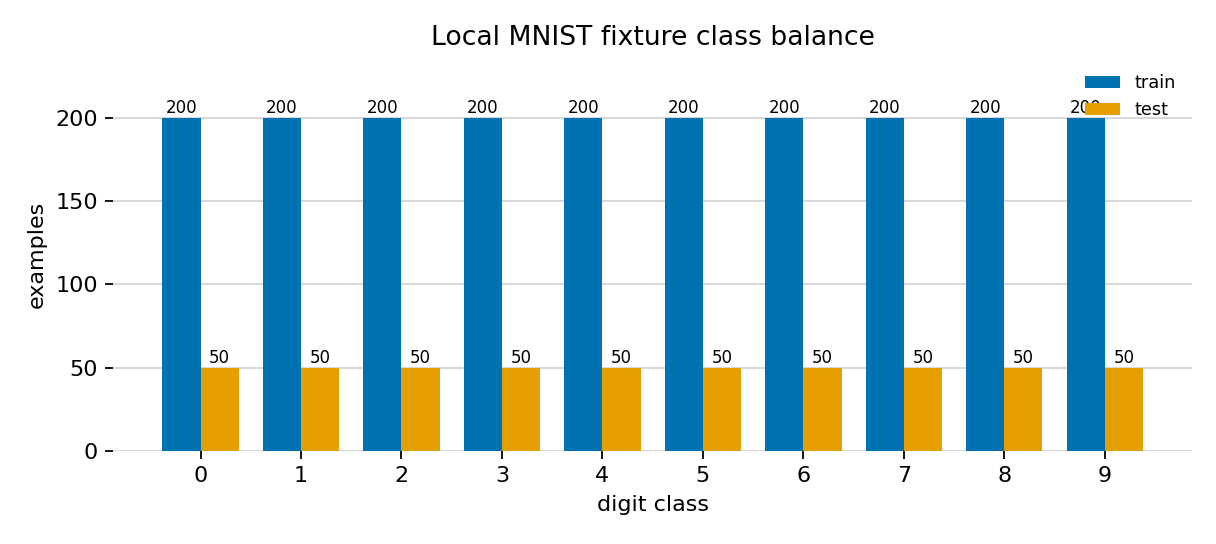
\includegraphics[keepaspectratio,alt={Train and test class counts from output/data/ml\_class\_balance.json; the local fixture contains 2000 train and 500 test examples across 10 classes. Generation method: Grouped train/test class-count bars from the local MNIST fixture. Registry metadata records the generation method, source artifact, and claim boundary for validation.}]{../figures/mnist_class_balance.png}}
\caption{Train and test class counts from
output/data/ml\_class\_balance.json; the local fixture contains 2000
train and 500 test examples across 10 classes. Generation method:
Grouped train/test class-count bars from the local MNIST fixture.
Registry metadata records the generation method, source artifact, and
claim boundary for validation.}\label{fig:mnist_class_balance}
\end{figure}

\begin{longtable}[]{@{}llll@{}}
\caption{Local fixture class-balance table from
\protect\breaktt{output/data/ml\_class\_balance.json}; counts describe
the offline fixture used by this
run.}\label{tbl:class-balance}\tabularnewline
\toprule\noalign{}
Split & Class & Count & Fraction \\
\midrule\noalign{}
\endfirsthead
\toprule\noalign{}
Split & Class & Count & Fraction \\
\midrule\noalign{}
\endhead
train & 0 & 200 & 10.0\% \\
train & 1 & 200 & 10.0\% \\
train & 2 & 200 & 10.0\% \\
train & 3 & 200 & 10.0\% \\
train & 4 & 200 & 10.0\% \\
train & 5 & 200 & 10.0\% \\
train & 6 & 200 & 10.0\% \\
train & 7 & 200 & 10.0\% \\
train & 8 & 200 & 10.0\% \\
train & 9 & 200 & 10.0\% \\
test & 0 & 50 & 10.0\% \\
test & 1 & 50 & 10.0\% \\
test & 2 & 50 & 10.0\% \\
test & 3 & 50 & 10.0\% \\
test & 4 & 50 & 10.0\% \\
test & 5 & 50 & 10.0\% \\
test & 6 & 50 & 10.0\% \\
test & 7 & 50 & 10.0\% \\
test & 8 & 50 & 10.0\% \\
test & 9 & 50 & 10.0\% \\
\bottomrule\noalign{}
\end{longtable}

\begin{figure}
\centering
\pandocbounded{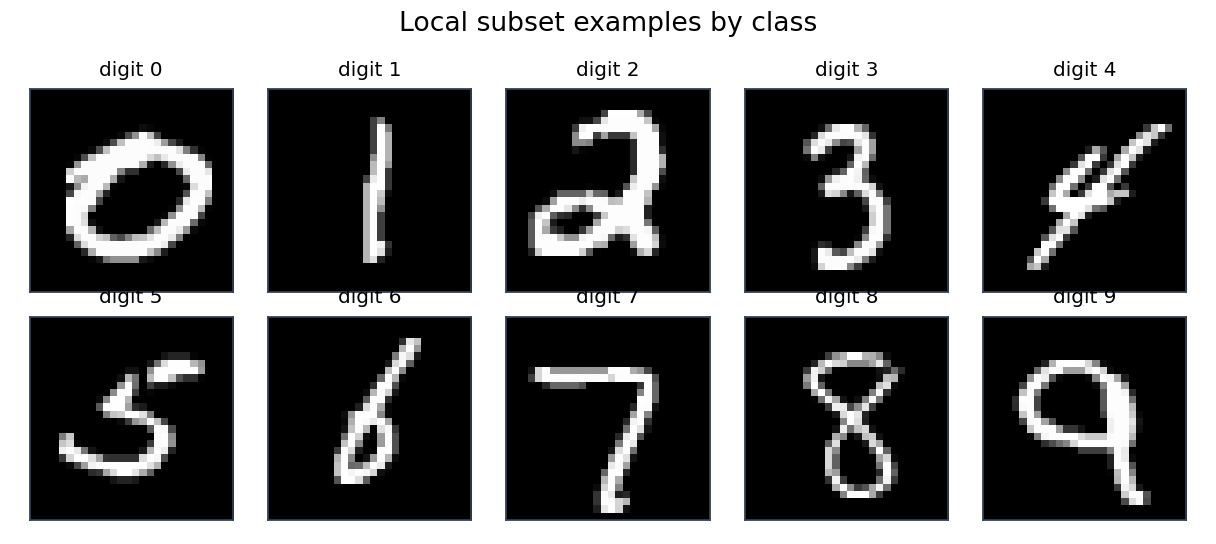
\includegraphics[keepaspectratio,alt={Deterministic class-balanced contact sheet for MNIST handwritten digit database from data/mnist\_small.npz and data/mnist\_small\_provenance.json; the figure documents the local subset used by the offline run. Generation method: Class-balanced contact sheet from fixed local MNIST arrays. Registry metadata records the generation method, source artifact, and claim boundary for validation.}]{../figures/mnist_subset_contact_sheet.png}}
\caption{Deterministic class-balanced contact sheet for MNIST
handwritten digit database from data/mnist\_small.npz and
data/mnist\_small\_provenance.json; the figure documents the local
subset used by the offline run. Generation method: Class-balanced
contact sheet from fixed local MNIST arrays. Registry metadata records
the generation method, source artifact, and claim boundary for
validation.}\label{fig:mnist_subset_contact_sheet}
\end{figure}

The baseline is \breaktt{nearest\_centroid\_baseline}
(\breaktt{nearest-centroid}). The bounded candidate set is configured by
the task artifact and covers
\breaktt{MLP,\ nearest-centroid,\ softmax\ regression,\ tiny\ patch-attention},
including \breaktt{Tiny\ patch-attention\ classifier} and at least one
deferred proposal. The transformer-style candidate borrows the
patch-token representation for comparison while staying inside the
configured iteration budget. This is intentionally a small configured
model, not a claim about full-scale image-transformer performance.
\end{frame}

\begin{frame}[fragile,allowframebreaks]{Bounded Loop}
\protect\phantomsection\label{sec:bounded-loop}
The run follows \texttt{7} configured stages:

\begin{itemize}
\tightlist
\item
  Resolve the human-authored program, project topic, and research
  questions.
\item
  Build an \breaktt{AutoResearchPlan} from the domain profile, experiment
  plan, and pipeline DAG.
\item
  Validate exact stage-gate names declared in
  \breaktt{autoresearch.yaml}.
\item
  Evaluate the configured \texttt{MNIST} candidate set up to the
  configured iteration budget.
\item
  Generate claims only from configured questions and local artifact
  paths.
\item
  Write data, reports, figures, benchmark scores, and review packets
  under the declared output contract.
\item
  Run strict AutoResearch readiness validation and write readiness
  reports.
\end{itemize}

Candidates are declared in the proposal ledger and resolved from the
task configuration for execution. Each executable candidate declares a
model type, seed, training schedule, and model-specific parameters. The
configured training policy includes learning-rate decay \texttt{0.995}
and gradient clipping norm \texttt{5}, both recorded from the validated
task run rather than described as a free-form manuscript setting. The
loop evaluates at most \texttt{4} configured iterations, selects the
highest \texttt{test\_accuracy}, and breaks ties by lower parameter
count and identifier. Candidates outside the budget are recorded as
deferred; the run-derived status summary is
\breaktt{accepted:\ 1,\ deferred:\ 1,\ rejected:\ 3}.

The closure is concrete and file-backed.
\breaktt{output/data/research\_program.json} constrains proposals;
proposal records feed the bounded evaluation; evaluation writes
\breaktt{output/data/ml\_candidate\_ledger.json} and
\breaktt{output/data/run\_ledger.json}; ledgers support artifact-linked
claims; claims hydrate the manuscript through
\breaktt{output/data/manuscript\_variables.json}; readiness validation
writes \breaktt{output/reports/autoresearch\_readiness.json}; loop
settlement is recorded in
\breaktt{output/data/autoresearch\_phase\_ledger.json}; and review state
is captured in \breaktt{output/data/review\_decisions.json}. The loop
therefore maintains an inspectable research process around a small
metric result without making the process self-approving or opaque.

The concrete closure is intentionally close to research-object and
workflow-run provenance practice. The artifact manifest lists generated
objects and checksums; the figure registry binds captions to source
artifacts; the variable provenance sidecar records the source pointer
for each injected token or table; and the review packet keeps human
decisions outside generated approval. This is a minimal local analogue
of machine-readable provenance rather than a claim of full
research-object packaging.

The generated schema manifest at
\breaktt{output/data/autoresearch\_schema\_manifest.json} records
\texttt{31} schema-versioned governance payload(s) plus documented
generic-table exemptions. The local research-object manifest at
\breaktt{output/data/research\_object\_manifest.json} packages observed
project paths, hashes, the evidence registry, the source ledger, the
schema manifest, and the manual approval state. It is deliberately named
a local research-object manifest, not RO-Crate or SLSA compliance.
\end{frame}

\begin{frame}[fragile,allowframebreaks]{Safety Controls}
\protect\phantomsection\label{sec:safety-controls}
The default autonomy level is \texttt{proposal\_only}. The run ledger
records \texttt{0} LLM calls and USD \texttt{0.00} cost. The edit
allowlist is restricted to the public project source and manuscript
surfaces, plus the task configuration file, and the pipeline never
executes generated code. Review gates are emitted with deferred
decisions so that validation can confirm the gates exist without
pretending that the machine approved publication.

Publication approval is a non-generated input. The run may read
\breaktt{human\_review.yaml} and copy its state into review payloads, but
generated readiness cannot set publication approval by itself; the
default local review state remains \texttt{false}.

Disclosure: \breaktt{AI-assisted\ AutoResearch} status is declared for
this exemplar because it models machine-produced plans, ledgers,
reports, and manuscript variables as review inputs rather than
autonomous approval.
\end{frame}

\begin{frame}[fragile,allowframebreaks]{Adversarial And Supply-Chain
Controls}
\protect\phantomsection\label{sec:adversarial-supply-chain-controls}
The security layer is configured as \breaktt{local\_deterministic} with
network policy \texttt{default\_offline}, integrity algorithm
\texttt{sha256}, external signing \texttt{false}, and framework labels
\breaktt{STRIDE,\ MITRE\_ATT\&CK\_T1195}. Its scope is
\breaktt{Local\ research-artifact\ integrity\ evidence\ for\ this\ deterministic\ public\ exemplar}.
These values are generated from
\breaktt{output/data/autoresearch\_security\_profile.json}; the default
run remains offline and deterministic.

The local threat model covers \texttt{7} asset(s), \texttt{7} threat
row(s), and \texttt{7} control row(s). The security artifacts are
written to \breaktt{output/data/autoresearch\_threat\_model.json},
\breaktt{output/data/autoresearch\_supply\_chain\_inventory.json},
\breaktt{output/data/autoresearch\_integrity\_attestation.json}, and
\breaktt{output/reports/autoresearch\_security\_review.md}. The
control-matrix figure is @fig:autoresearch\_security\_control\_matrix.
The table and figure are generated from the threat model and inventory,
not manually maintained.

\begin{figure}
\centering
\pandocbounded{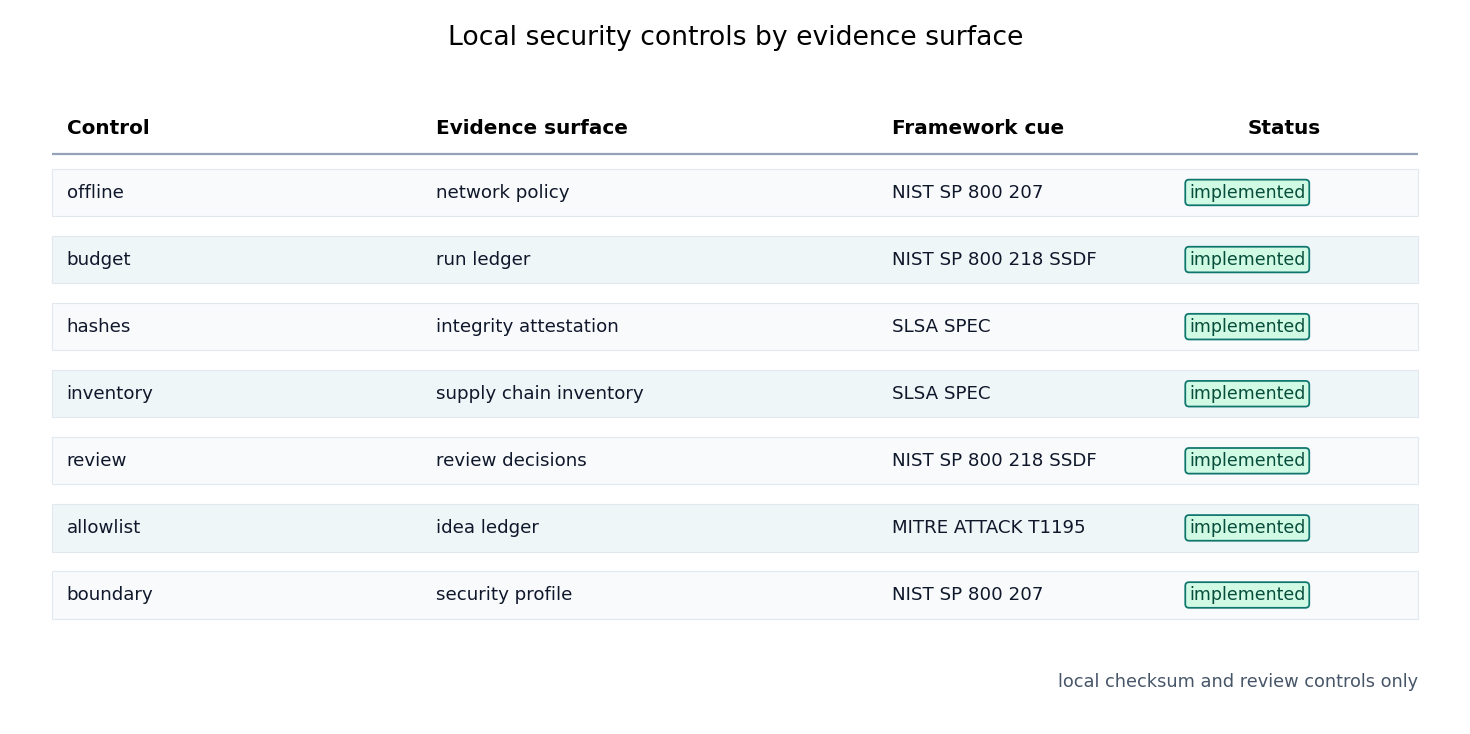
\includegraphics[keepaspectratio,alt={Local security-control matrix from output/data/autoresearch\_threat\_model.json; controls map NIST, SLSA, and ATT\&CK-inspired safeguards to deterministic evidence surfaces without claiming production security certification. Generation method: structured control matrix with separate control, evidence, framework, and status columns. Generation method: Structured control matrix from local threat-model controls. Registry metadata records the generation method, source artifact, and claim boundary for validation.}]{../figures/autoresearch_security_control_matrix.png}}
\caption{Local security-control matrix from
output/data/autoresearch\_threat\_model.json; controls map NIST, SLSA,
and ATT\&CK-inspired safeguards to deterministic evidence surfaces
without claiming production security certification. Generation method:
structured control matrix with separate control, evidence, framework,
and status columns. Generation method: Structured control matrix from
local threat-model controls. Registry metadata records the generation
method, source artifact, and claim boundary for
validation.}\label{fig:autoresearch_security_control_matrix}
\end{figure}

\begin{longtable}[]{@{}
  >{\raggedright\arraybackslash}p{(\linewidth - 4\tabcolsep) * \real{0.3333}}
  >{\raggedright\arraybackslash}p{(\linewidth - 4\tabcolsep) * \real{0.3333}}
  >{\raggedright\arraybackslash}p{(\linewidth - 4\tabcolsep) * \real{0.3333}}@{}}
\caption{Local security artifacts generated for the bounded AutoResearch
run.}\label{tbl:security-artifacts}\tabularnewline
\toprule\noalign{}
\begin{minipage}[b]{\linewidth}\raggedright
Security artifact
\end{minipage} & \begin{minipage}[b]{\linewidth}\raggedright
Path
\end{minipage} & \begin{minipage}[b]{\linewidth}\raggedright
Summary
\end{minipage} \\
\midrule\noalign{}
\endfirsthead
\toprule\noalign{}
\begin{minipage}[b]{\linewidth}\raggedright
Security artifact
\end{minipage} & \begin{minipage}[b]{\linewidth}\raggedright
Path
\end{minipage} & \begin{minipage}[b]{\linewidth}\raggedright
Summary
\end{minipage} \\
\midrule\noalign{}
\endhead
profile & \href{../data/autoresearch_security_profile.json}{security
profile} & local\_deterministic \\
threat model & \href{../data/autoresearch_threat_model.json}{threat
model} & default\_offline \\
inventory &
\href{../data/autoresearch_supply_chain_inventory.json}{supply
inventory} & 14 inputs \\
inventory export &
\href{../data/autoresearch_inventory_export.json}{inventory export} &
local non-SBOM export \\
attestation &
\href{../data/autoresearch_integrity_attestation.json}{integrity
attestation} & passed \\
review & \href{../reports/autoresearch_security_review.md}{security
review} & human review input \\
\bottomrule\noalign{}
\end{longtable}

\begingroup\footnotesize

\begin{longtable}[]{@{}
  >{\raggedright\arraybackslash}p{(\linewidth - 8\tabcolsep) * \real{0.2000}}
  >{\raggedright\arraybackslash}p{(\linewidth - 8\tabcolsep) * \real{0.2000}}
  >{\raggedright\arraybackslash}p{(\linewidth - 8\tabcolsep) * \real{0.2000}}
  >{\raggedright\arraybackslash}p{(\linewidth - 8\tabcolsep) * \real{0.2000}}
  >{\raggedright\arraybackslash}p{(\linewidth - 8\tabcolsep) * \real{0.2000}}@{}}
\caption{Threat-model rows from
\protect\breaktt{output/data/autoresearch\_threat\_model.json}; ATT\&CK
labels scope supply-chain compromise
analogies.}\label{tbl:security-threat-model}\tabularnewline
\toprule\noalign{}
\begin{minipage}[b]{\linewidth}\raggedright
Threat
\end{minipage} & \begin{minipage}[b]{\linewidth}\raggedright
STRIDE
\end{minipage} & \begin{minipage}[b]{\linewidth}\raggedright
ATT\&CK
\end{minipage} & \begin{minipage}[b]{\linewidth}\raggedright
Scenario
\end{minipage} & \begin{minipage}[b]{\linewidth}\raggedright
Residual risk
\end{minipage} \\
\midrule\noalign{}
\endfirsthead
\toprule\noalign{}
\begin{minipage}[b]{\linewidth}\raggedright
Threat
\end{minipage} & \begin{minipage}[b]{\linewidth}\raggedright
STRIDE
\end{minipage} & \begin{minipage}[b]{\linewidth}\raggedright
ATT\&CK
\end{minipage} & \begin{minipage}[b]{\linewidth}\raggedright
Scenario
\end{minipage} & \begin{minipage}[b]{\linewidth}\raggedright
Residual risk
\end{minipage} \\
\midrule\noalign{}
\endhead
dataset tamper & Tampering & T1195 & A local fixture could be replaced
or edited before analysis. & Residual risk remains if a reviewer ignores
checksum drift. \\
config drift & Tampering & T1195.001 & Task settings could silently
change candidate scope, budgets, or diag\ldots{} & Configuration review
is still a human responsibility. \\
source edit & Elevation of privilege & T1195.001 & Source changes could
bypass the thin-script and no-generated-code bou\ldots{} & The default
run does not perform full static application security tes\ldots{} \\
output tamper & Repudiation & T1195.002 & Generated reports or figures
could be edited after analysis but befor\ldots{} & Local checksum
evidence is not externally signed. \\
manuscript injection & Information disclosure & T1195.002 & Manual prose
could hard-code run facts that bypass validated variables. & Stable
scholarly prose and citekeys remain manually authored. \\
self approval & Spoofing & T1195 & Generated review packets could be
mistaken for human publication appr\ldots{} & Publication remains
outside the automated loop. \\
build assumption & Denial of service & T1195.003 & A local or CI build
context could omit checks or run stale generated\ldots{} & The exemplar
does not sign build logs or isolate runners. \\
\bottomrule\noalign{}
\end{longtable}

\endgroup
\end{frame}

\begin{frame}[allowframebreaks]{Positioning Against Autonomous Science
Systems}
\protect\phantomsection\label{sec:positioning-autonomous-science}
The implementation should be read as a bounded local analogue of current
AutoResearch trends, not as a miniature autonomous scientist. Artifact
manifests, evidence registries, review gates, and manuscript hydration
provide machine-readable governance surfaces for one offline project
run. They do not perform autonomous literature mining, proof search,
live agent orchestration, runtime dataset expansion, self-modifying code
search, or self-approval of publication claims.
\end{frame}

\begin{frame}[fragile,allowframebreaks]{Evidence And Scoring}
\protect\phantomsection\label{sec:evidence-scoring}
The experiment writes \breaktt{output/data/ml\_task\_results.json},
\breaktt{output/data/ml\_candidate\_ledger.json},
\breaktt{output/data/ml\_confusion\_matrix.csv},
\breaktt{output/data/ml\_training\_history.csv},
\breaktt{output/data/ml\_error\_examples.json},
\breaktt{output/data/ml\_prediction\_records.json},
\breaktt{output/data/ml\_classification\_diagnostics.json},
\breaktt{output/data/ml\_candidate\_intervals.json},
\breaktt{output/data/ml\_class\_balance.json},
\breaktt{output/data/ml\_calibration\_report.json},
\breaktt{output/data/ml\_calibration\_bin\_intervals.json},
\breaktt{output/data/ml\_robustness\_report.json},
\breaktt{output/data/ml\_probability\_diagnostics.json},
\breaktt{output/data/ml\_bootstrap\_intervals.json},
\breaktt{output/data/ml\_paired\_comparison.json},
\breaktt{output/data/ml\_candidate\_rank\_stability.json},
\breaktt{output/data/ml\_statistical\_summary.json},
\breaktt{output/data/ml\_training\_diagnostics.json},
\breaktt{output/reports/ml\_benchmark\_score.json},
\breaktt{output/data/benchmark\_boundary.json},
\breaktt{output/data/figure\_quality\_report.json}, and registered
figures through \breaktt{output/figures/figure\_registry.json}. The
diagnostic payloads preserve probabilities, confidence and margin
summaries, class metrics, calibration bins, confusion-pair summaries,
train/test gaps, deterministic no-retrain perturbation scores, bootstrap
intervals, paired baseline comparison, rank-stability frequencies,
calibration-bin Wilson intervals, selective accuracy thresholds, Brier
score, negative log likelihood, top-2 accuracy, probability-quality
comparisons, learning-rate traces, best-epoch markers, final learning
rates, and train-test gap summaries without serializing model weights.
The benchmark score combines metric improvement, budget compliance,
offline execution, transformer-candidate coverage, and
candidate-selection status. The benchmark-boundary artifact records
fixture scope, metric direction, candidate families, budget,
statistical-method artifacts, and explicit non-claims, so
benchmark-adjacent statistics remain local readiness diagnostics rather
than broad empirical or publication claims. Manuscript variables are
hydrated from these artifacts, and readiness validation checks
\breaktt{output/reports/evidence\_registry.json},
\breaktt{output/reports/artifact\_manifest.json}, method ledgers, review
gates, benchmark outputs, the phase ledger, figure-quality report, and
AI-assisted disclosure before rendering is treated as ready for review.
The reviewer-facing
\breaktt{output/data/autoresearch\_evidence\_overview.json} then
summarizes readiness versus publication approval, claim-evidence rows,
source-ledger status, benchmark boundary issues, and security/integrity
status without granting approval. The generated tables and figure blocks
used in @sec:results are sourced through
\breaktt{output/data/manuscript\_variable\_provenance.json} and
\breaktt{output/data/manuscript\_figure\_blocks.json}, so captions,
artifact tables, and run-derived result statements share the same
validated artifact base.

The figure registry also carries the method contract for each
visualization: source artifact, generated file, rendering method, and
claim boundary. The rendered method table below is generated from that
registry rather than maintained manually.

\begingroup\footnotesize

\begin{longtable}[]{@{}
  >{\raggedright\arraybackslash}p{(\linewidth - 6\tabcolsep) * \real{0.2500}}
  >{\raggedright\arraybackslash}p{(\linewidth - 6\tabcolsep) * \real{0.2500}}
  >{\raggedright\arraybackslash}p{(\linewidth - 6\tabcolsep) * \real{0.2500}}
  >{\raggedright\arraybackslash}p{(\linewidth - 6\tabcolsep) * \real{0.2500}}@{}}
\caption{Registry-backed figure methods from
\href{../figures/figure_registry.json}{\protect\breaktt{figure\_registry.json}};
full validation hooks, alt text, and claim boundaries remain in the
registry.}\label{tbl:figure-methods}\tabularnewline
\toprule\noalign{}
\begin{minipage}[b]{\linewidth}\raggedright
Figure
\end{minipage} & \begin{minipage}[b]{\linewidth}\raggedright
Source
\end{minipage} & \begin{minipage}[b]{\linewidth}\raggedright
Method
\end{minipage} & \begin{minipage}[b]{\linewidth}\raggedright
Scope
\end{minipage} \\
\midrule\noalign{}
\endfirsthead
\toprule\noalign{}
\begin{minipage}[b]{\linewidth}\raggedright
Figure
\end{minipage} & \begin{minipage}[b]{\linewidth}\raggedright
Source
\end{minipage} & \begin{minipage}[b]{\linewidth}\raggedright
Method
\end{minipage} & \begin{minipage}[b]{\linewidth}\raggedright
Scope
\end{minipage} \\
\midrule\noalign{}
\endhead
@fig:autoresearch\_candidate\_lifecycle &
\href{../data/ml_candidate_ledger.json}{candidate ledger} & Candidate
lifecycle status-count bar chart. & Lifecycle counts describe bounded
orchestration, not autonomous approval. \\
@fig:autoresearch\_closure\_flow &
\href{../data/autoresearch_loop.json}{loop} & File-backed process-flow
diagram from final loop state. & The workflow is file-backed and
inspectable but not self-approving. \\
@fig:autoresearch\_integrity\_chain &
\href{../data/autoresearch_integrity_attestation.json}{integrity
attestation} & Local checksum attestation chain with checked, missing,
and mismatch counts. & Integrity checks are local SHA-256 observations
and are not externally signed provenance. \\
@fig:autoresearch\_security\_control\_matrix &
\href{../data/autoresearch_threat_model.json}{threat model} & Structured
control matrix from local threat-model controls. & Controls are local
research-artifact safeguards, not production security certification. \\
@fig:autoresearch\_stage\_matrix &
\href{../data/autoresearch_loop.json}{loop} & Horizontal count summary
from final loop metrics. & Readiness artifacts summarize local
validation only; publication approval is human. \\
@fig:ml\_bootstrap\_intervals &
\href{../data/ml_bootstrap_intervals.json}{bootstrap intervals} &
Horizontal percentile-bootstrap interval plot. & Bootstrap intervals
summarize local test-set resampling only. \\
@fig:ml\_calibration\_reliability &
\href{../data/ml_calibration_report.json}{calibration report} &
Reliability curve with confidence-bin support histogram. & Calibration
values describe the fixed local split only. \\
@fig:ml\_candidate\_rank\_stability &
\href{../data/ml_candidate_rank_stability.json}{candidate rank
stability} & Bootstrap top-rank frequency and mean-rank comparison. &
Rank stability describes local resampling behavior, not model-selection
certainty. \\
@fig:ml\_candidate\_scores &
\href{../data/ml_candidate_intervals.json}{candidate intervals} &
Lollipop accuracy comparison with Wilson interval error bars and direct
labels. & Scores apply only to the fixed local subset and configured
candidates. \\
@fig:ml\_classification\_metrics\_heatmap &
\href{../data/ml_classification_diagnostics.json}{class diagnostics} &
Per-class precision, recall, and F1 heatmap. & Class metrics diagnose
this run only and are not full-dataset estimates. \\
@fig:ml\_complexity\_accuracy & \href{../data/ml_task_results.json}{task
results} & Log-parameter scatter plot against held-out accuracy. & The
plot compares this bounded candidate set and does not infer a scaling
law. \\
@fig:ml\_confusion\_matrix &
\href{../data/ml_confusion_matrix.csv}{confusion matrix} &
Row-normalized heatmap with cell counts and row percentages. & Confusion
counts diagnose this run only and do not imply full-dataset
generalization. \\
@fig:ml\_confusion\_pairs &
\href{../data/ml_classification_diagnostics.json}{class diagnostics} &
Ranked off-diagonal confusion-pair bars with true-class error rates. &
Pair counts identify local error cases and are not a general
taxonomy. \\
@fig:ml\_generalization\_gap &
\href{../data/ml_classification_diagnostics.json}{class diagnostics} &
Grouped train/test accuracy and loss bars by evaluated candidate. & Gaps
are local bounded-loop diagnostics, not convergence guarantees. \\
@fig:ml\_learning\_curves &
\href{../data/ml_training_history.csv}{training history} & Epoch-level
held-out accuracy lines with accepted best-epoch marker. & Learning
curves diagnose configured training only, not convergence in general. \\
@fig:ml\_paired\_correctness &
\href{../data/ml_paired_comparison.json}{paired comparison} & Matched
accepted-versus-baseline correctness heatmap. & Matched comparison is
limited to the fixed local test split. \\
@fig:ml\_per\_class\_accuracy &
\href{../data/ml_confusion_matrix.csv}{confusion matrix} & Per-class
accuracy bars computed from the confusion matrix diagonal. & Per-class
values diagnose this local split only and do not certify robustness. \\
@fig:ml\_probability\_margin\_distribution &
\href{../data/ml_probability_diagnostics.json}{probability diagnostics}
& Confidence and margin histograms split by correctness. & Distributions
are descriptive diagnostics for the fixed local test split. \\
@fig:ml\_probability\_quality &
\href{../data/ml_statistical_summary.json}{statistical summary} & Brier
score and negative-log-likelihood bar comparison. & Probability-quality
metrics compare the configured evaluated candidates only. \\
@fig:ml\_robustness\_matrix &
\href{../data/ml_robustness_report.json}{robustness report} &
Candidate-by-transform accuracy heatmap for deterministic perturbations.
& Deterministic perturbations are a smoke test and do not certify
robustness. \\
@fig:ml\_selective\_accuracy &
\href{../data/ml_statistical_summary.json}{statistical summary} &
Confidence-threshold coverage and selective-accuracy line chart. &
Selective accuracy describes thresholded predictions on the fixed local
split only. \\
@fig:ml\_training\_dynamics &
\href{../data/ml_training_diagnostics.json}{training diagnostics} &
Final and best-epoch accuracy bars plus train-test gap bars. & Training
dynamics diagnose this configured deterministic run only. \\
@fig:mnist\_class\_balance & \href{../data/ml_class_balance.json}{class
balance} & Grouped train/test class-count bars from the local MNIST
fixture. & Class counts describe the local fixed fixture and are not
population statistics. \\
@fig:mnist\_error\_examples &
\href{../data/ml_error_examples.json}{error examples} & Deterministic
grid of the first accepted-candidate misclassifications. & Examples are
qualitative diagnostics for this run, not an error taxonomy. \\
@fig:mnist\_subset\_contact\_sheet &
\href{../../data/mnist_small.npz}{small} & Class-balanced contact sheet
from fixed local MNIST arrays. & The sheet illustrates the local fixed
subset and is not a statistical sample claim. \\
\bottomrule\noalign{}
\end{longtable}

\endgroup
\end{frame}

\end{document}
